% {\color{blue} 초안 작성 v0.1}

% {\color{blue} 결과 쉽게 풀어쓰도록 수정}

\section{Experiment Setup}
\label{sec:eval-experiment-setup}
RL-SchedExt는 Google Pixel 9 Pro XL (Google Tensor G4)의 AOSP Android 15
(\texttt{android-15.0.0\_r36}) 환경에서 평가하였다. Linux 6.1 기반 Android
Kernel에 Linux 6.12의 sched\_ext를 Backport하였으며, 해당 환경의 기본
Fair Scheduler인 CFS를 Baseline으로 사용하였다~\cite{cfs,pixelkernel}.
EEVDF는 이후 Linux 버전에서 도입된 방식이므로 본 실험의 Baseline에는 포함하지 않았다.

Microbenchmark에서는 Task Ordering의 효과를 독립적으로 평가하고 실험의
반복성과 측정 결과의 안정성을 확보하기 위해 모든 benchmark worker thread의
CPU Affinity를 Big Core인 CPU7로 고정하였다. 이를 통해 단일 CPU에서
경쟁하는 Task의 실행 순서를 평가하고, Core 간 Migration 및 이종 Core의
성능 차이에 의한 영향을 배제하였다. 또한 Dynamic Voltage and Frequency Scaling (DVFS)의 CPU Frequency Governor를
\texttt{performance}로 설정하여 주파수 변동이 측정 결과에 미치는 영향을
최소화하였다.

비교 대상은 CFS, Linear Student를 적용한 RL-SchedExt 구성, Neural Student를 적용한 RL-SchedExt 구성의 총 세 가지이다.
Linear Student는 Knowledge Distillation을 통해 RL Teacher의 Scheduling Policy를 학습한 선형 비교 모델이며,
Neural Student는 제안하는 경량 DeepSets 기반 모델이다.
이후 Microbenchmark와 Scheduling Policy Analysis에서는 세 실험군을 CFS, Linear Student, Neural Student로 표기한다.
Macrobenchmark와 전체 시스템의 성능을 설명할 때 RL-SchedExt는 Neural Student를 적용한 제안 구성을 의미한다.
두 Student는 동일한 57차원 State를 입력받고 Learned Vruntime Adjustment를 계산하여
Urgency-aware Vruntime을 기준으로 Task Ordering을 결정한다.
따라서 두 Student의 비교를 통해 입력 정보와 Task Ordering 방식이 동일한 조건에서
학습된 Scheduling Policy의 표현력이 성능에 미치는 영향을 조사한다.

Macrobenchmark에서는 실제 Android 게임의
frame 출력 성능을 별도로 평가하였다.

\section{Microbenchmark}
\label{sec:eval-microbenchmark}
\subsection{Workloads and Methodology}
\label{sec:eval-workloads-and-methodology}
Task Ordering의 성능을 평가하기 위해 CPU7에서 실행되는 세 가지 Workload를 사용하였다. 
\begin{itemize}
    \item \textit{Mixed CPU Bursts}: 짧고 빈번한 Wakeup과 긴 CPU Burst를 가진 Task가 CPU 자원을 공유하는 상황을 구성한다.

    \item \textit{Lock Dependency}: Mutex를 보유한 Task와 이를 기다리는 Task 사이의 Dependency를 모사한다.

    \item \textit{Workload Transition}: 총 6개의 Phase에 걸쳐
    Periodic Request, Chained Request, Lock-dependent Request 및 CPU-intensive Request의 상대적인 발생 빈도가 변화하는 환경을 구성한다.
\end{itemize}

모든 Scheduler에는 동일한 Request Arrival과 CPU Demand를 정의한 사전 생성 Manifest를 사용하였다.
각 Scheduler와 Workload의 조합에 대해 동일한 Manifest를 사용하여 100회
반복 측정하였다. Application Request의 실제 Deadline은 Scheduling Policy에
제공하지 않고 성능 평가에만 활용하였다.
Figure~\ref{fig:sched-microbenchmark}(\subref{fig:sched-deadline})--(\subref{fig:sched-p99})에서는
각 지표의 평균과 Standard Deviation(SD)을 계산하였다.

평가 지표는 Background에서 정의한 Request-Level Deadline 지표를 바탕으로 Deadline Miss Count, Total Deadline Overrun 및 Request Completion Latency p99로 구성하였다. 
Deadline Miss Count는 Deadline을 초과한 Request의 개수이며, Total Deadline Overrun은 각 Request가 Absolute Deadline을 초과한 시간의 합이다. 
Request Completion Latency p99는 전체 Request의
Arrival Time부터 Completion Time까지의 지연 시간 분포의 99번째
백분위수로, Tail Latency 특성을 나타낸다.

\subsection{Deadline Compliance}
\label{sec:eval-deadline-compliance}
Figure~\ref{fig:sched-microbenchmark}(\subref{fig:sched-deadline})은 세 가지 Workload에서 측정한 실험군별
Deadline Miss Count를 비교한다. Neural Student는 CFS 대비 Mixed CPU Bursts에서 19.4\%, Lock Dependency에서 26.8\%, Workload Transition에서 22.6\%의 Deadline Miss Count 감소를 보였다. 
반면 Linear Student의 Deadline Miss Count 감소율은 동일한 Workload에서 각각 3.3\%, 7.3\%, 8.5\%로 상대적으로 작게 나타났다.

% Evaluation plots: pre-rendered PNG (600 DPI), shared grayscale legend.
\begin{figure}[H]
  \centering
  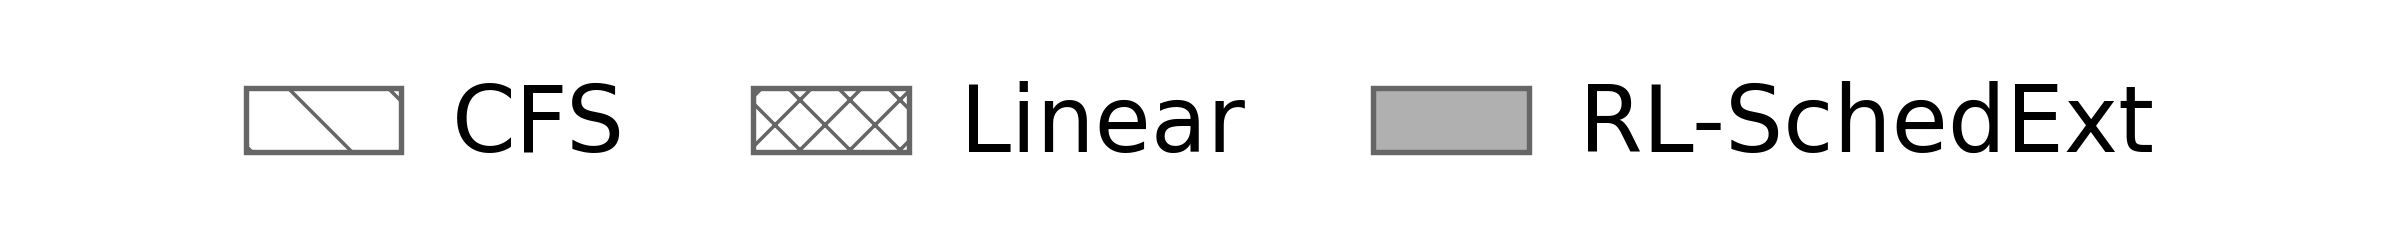
\includegraphics[width=0.50\linewidth]{Figures/fig5_1_legend.png}\par\smallskip
  \captionsetup[subfigure]{font=footnotesize,skip=3pt}
  \begin{subfigure}[b]{0.32\linewidth}
    \centering
    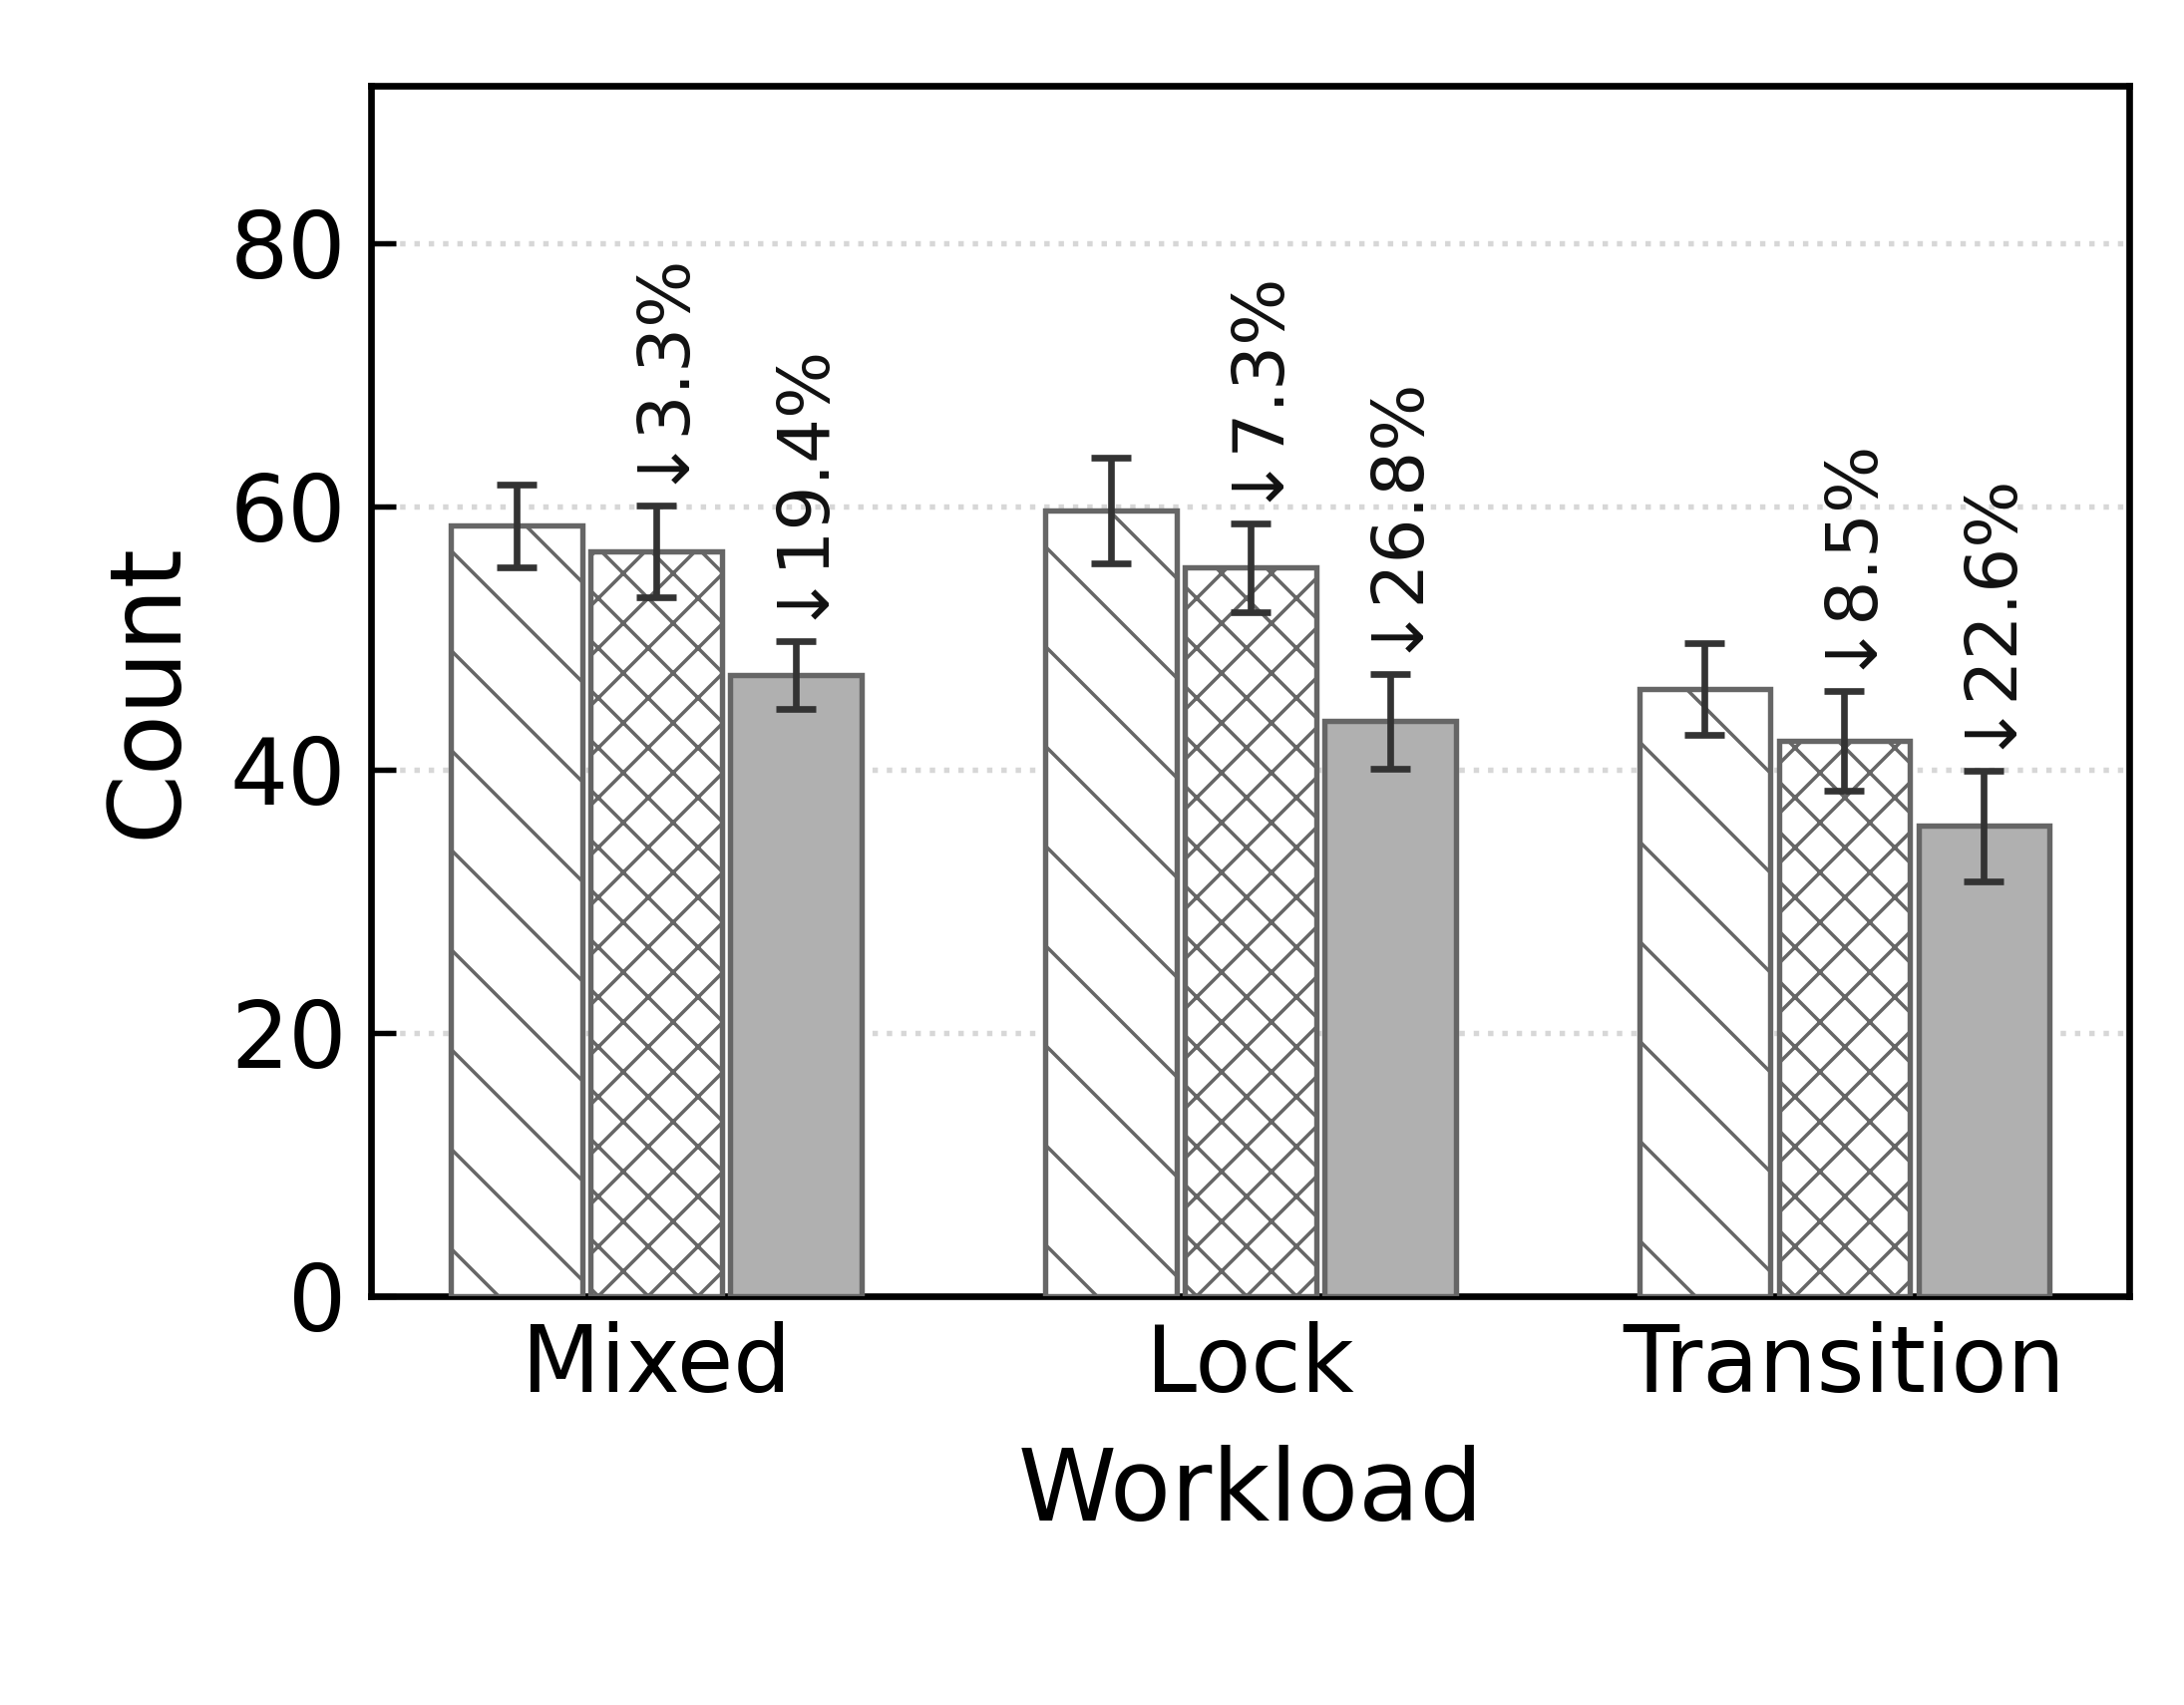
\includegraphics[width=\linewidth]{Figures/fig5_1_a_deadline_miss.png}
    \caption{Deadline miss count}
    \label{fig:sched-deadline}
  \end{subfigure}
  % \hspace{2pt}%
  \begin{subfigure}[b]{0.32\linewidth}
    \centering
    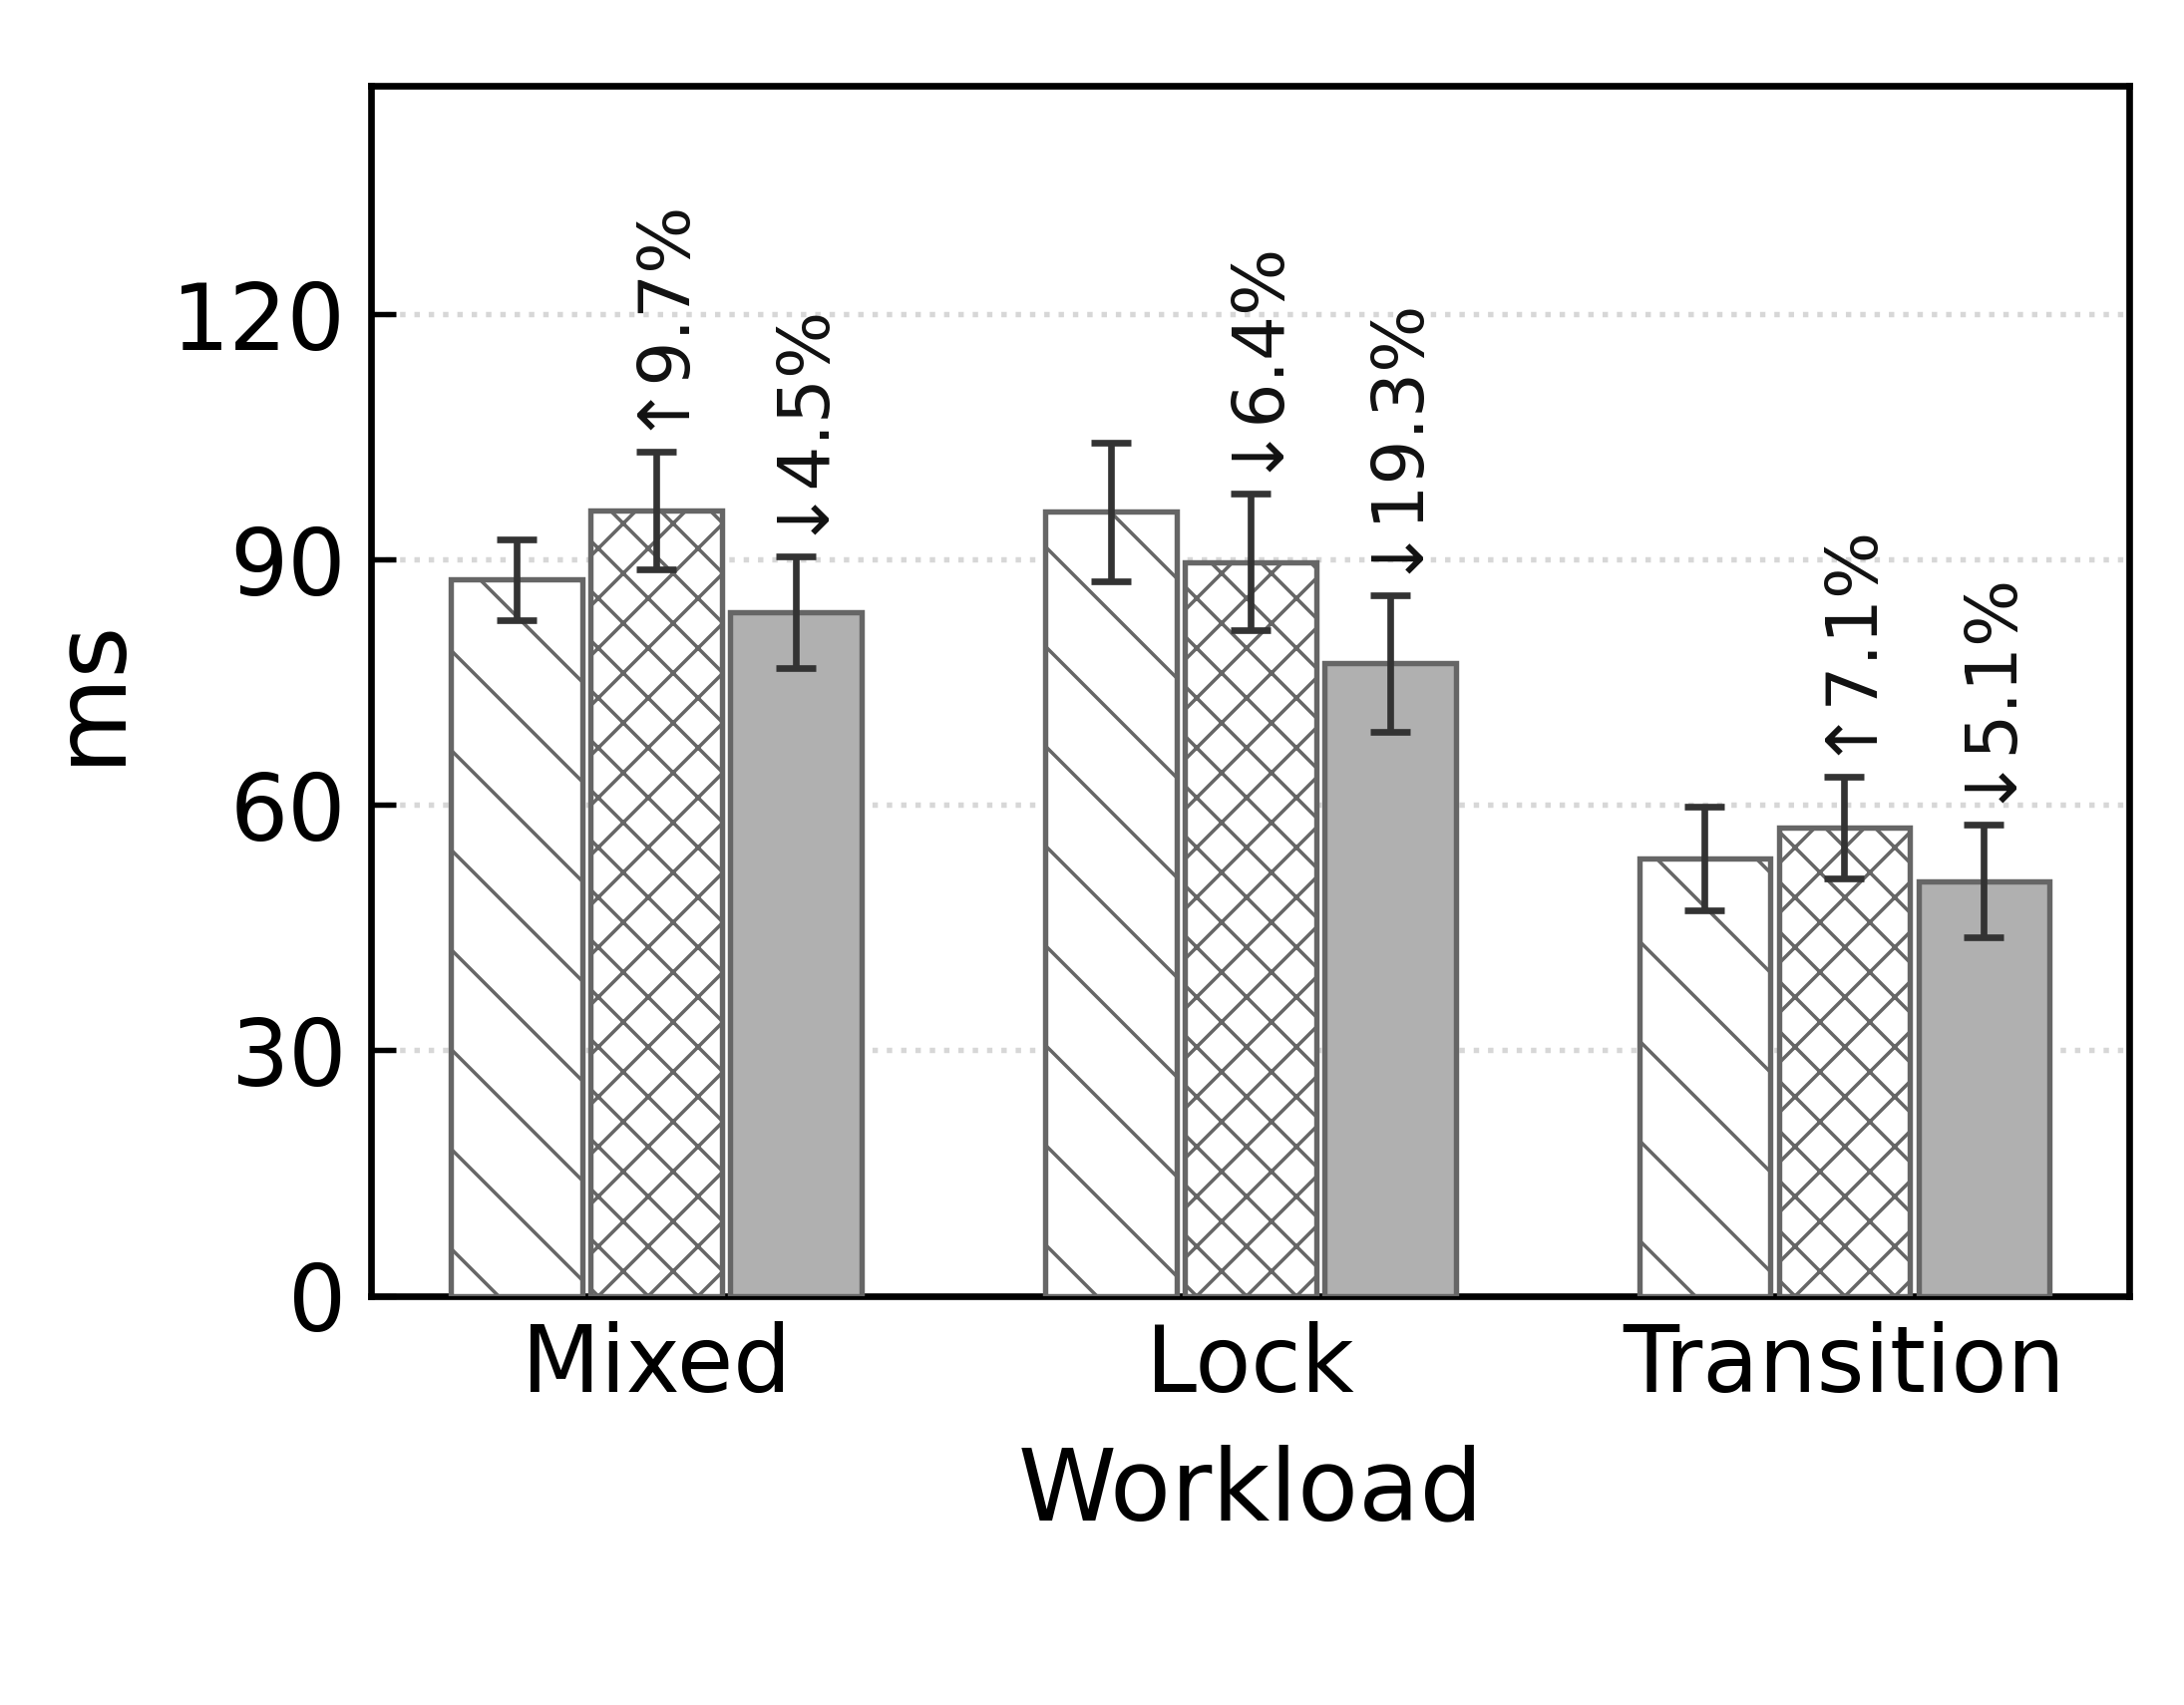
\includegraphics[width=\linewidth]{Figures/fig5_1_b_deadline_overrun.png}
    \caption{Total deadline overrun}
    \label{fig:sched-overrun}
  % \end{subfigure}\par\medskip
    \end{subfigure}
  \begin{subfigure}[b]{0.32\linewidth}
    \centering
    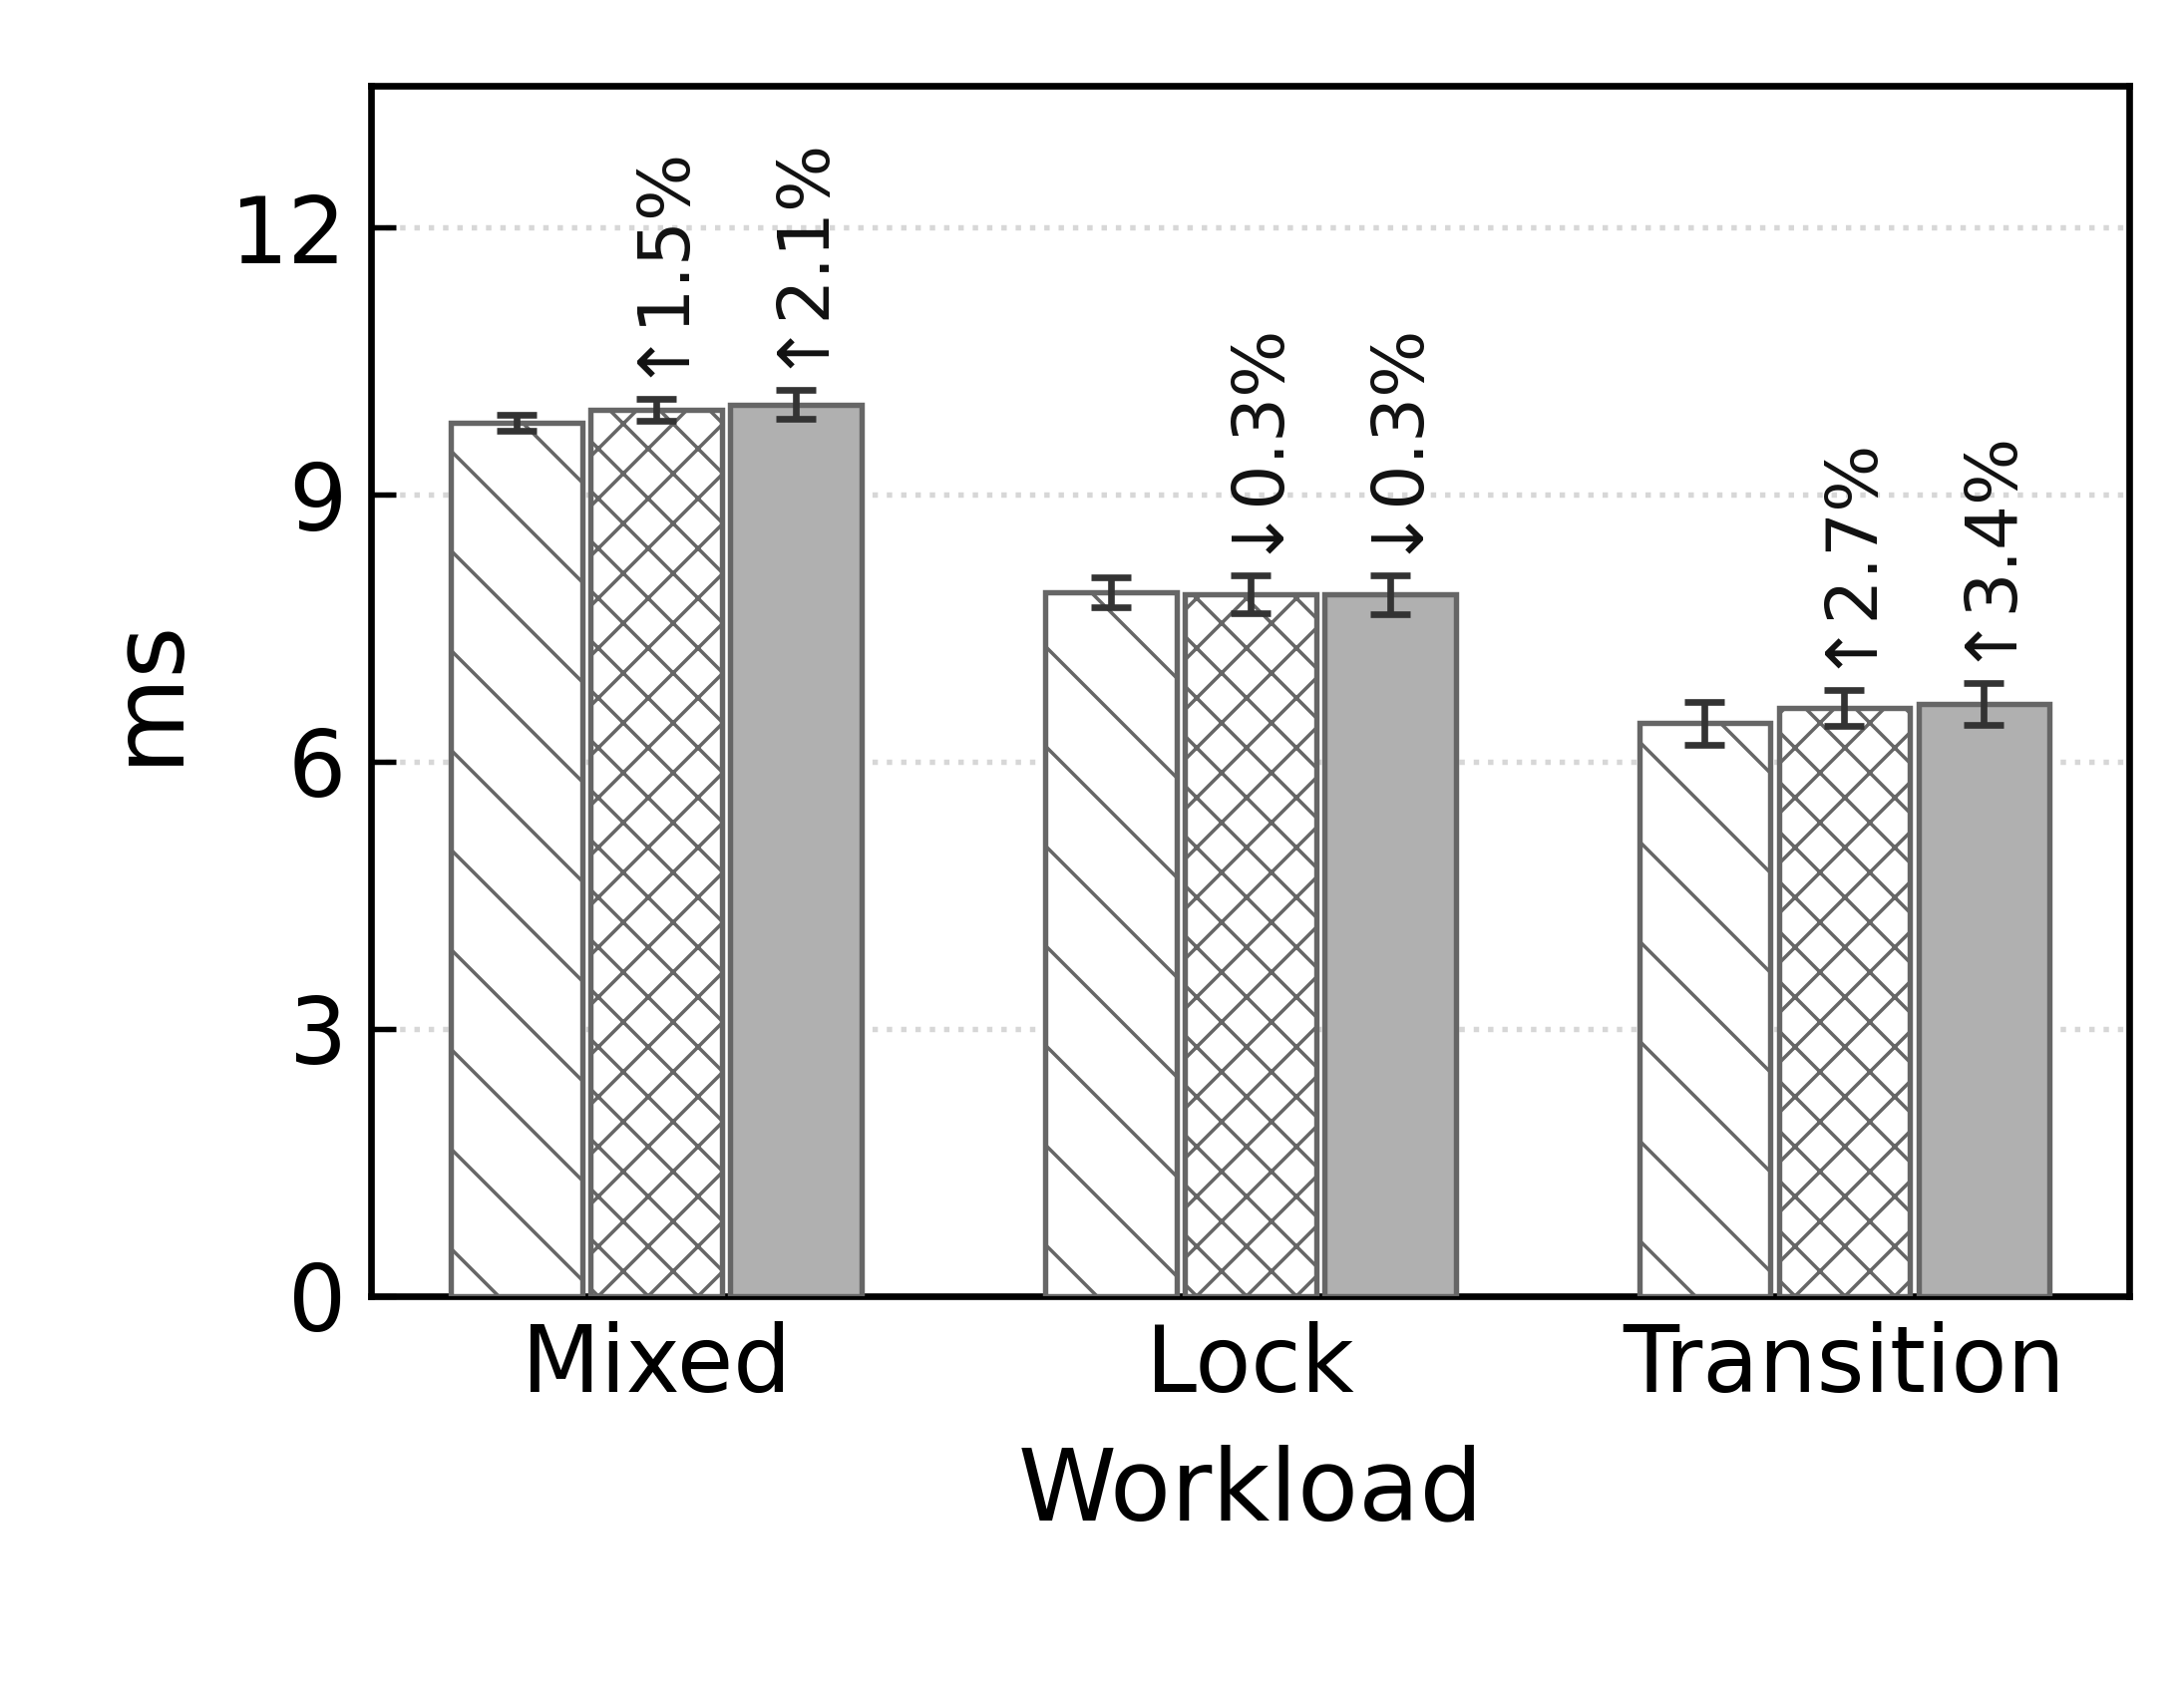
\includegraphics[width=\linewidth]{Figures/fig5_1_c_request_p99.png}
    \caption{Request latency p99}
    \label{fig:sched-p99}
  \end{subfigure}
  \caption{Pixel CPU7에서 수행한 Microbenchmark 결과. (a)--(c)는 Mixed CPU Bursts (Mixed), Lock Dependency (Lock), Workload Transition (Transition)의 성능을 비교한다. 각 지표별로 100회 측정 결과 중 상위 및 하위 5회를 제외한 90회의 결과를 사용하였다. 오차 막대는 표본 표준편차를 나타내며, 화살표는 CFS 대비 변화율을 나타낸다.}
  \label{fig:sched-microbenchmark}
\end{figure}


이러한 결과는 Neural Student가 평가한 세 가지 Workload 모두에서 Linear Student 및 CFS보다 낮은 Deadline Miss Count를 달성했음을 보여준다. 
특히 Mutex를 사용하는 Task 간 의존성이 존재하는 Lock Dependency에서 가장 큰 상대적 개선이 관찰되었다.

\subsection{Deadline Overrun and Tail Latency}
\label{sec:eval-deadline-overrun-and-tail-latency}
Figure~\ref{fig:sched-microbenchmark}(\subref{fig:sched-overrun})은 각 Workload에서 발생한 Total Deadline Overrun을 비교한다. 
Neural Student는 CFS 대비 Mixed CPU Bursts에서 4.5\%, Lock Dependency에서 19.3\%, Workload Transition에서 5.1\%의 Total Deadline Overrun 감소를 기록하였다.

반면 Linear Student는 Mixed CPU Bursts와 Workload Transition에서 각각 9.7\%, 7.1\%의 Total Deadline Overrun 증가를 보였으며, Lock Dependency에서는 6.4\% 감소하였다. 
이러한 결과는 Deadline Miss Count의 감소가 반드시 Total Deadline Overrun의 감소로 이어지는 것은 아님을 보여준다.
즉, Deadline을 놓친 Request의 개수뿐 아니라 개별 Request가 Deadline을 얼마나 초과했는지도 Scheduling Policy의 성능을 평가하는 데 중요한 요소이다.

Figure~\ref{fig:sched-microbenchmark}(\subref{fig:sched-p99})에서 Neural Student의 전체 Request Completion Latency p99는 CFS 대비 Mixed CPU Bursts에서 2.1\%, Workload Transition에서 3.4\% 증가하였으며, Lock Dependency에서는 약 0.3\% 감소하였다. 

Neural Student는 모든 Request의 Completion Latency를 균일하게 줄이기보다는 Scheduling Urgency가 높은 Task를 먼저 실행하도록 Task Ordering을 조정한다. 
그 과정에서 상대적으로 Urgency가 낮은 Task의 CPU 실행 기회가 늦어져 일부 Request의 Completion Latency가 증가할 수 있다. 
이러한 trade-off가 실제 성능에 어떻게 나타나는지 확인하기 위해 다음에서 Deadline Budget별 Request Completion Latency를 분석한다.

\section{Scheduling Policy Analysis}
\label{sec:eval-scheduling-policy-analysis}

\subsection{Latency Redistribution}
\label{sec:eval-latency-redistribution}
앞선 실험에서 Neural Student는 Deadline Compliance를 향상시켰으나,
일부 Workload에서는 전체 Request Completion Latency p99가 증가하였다.
이러한 Latency 증가가 Scheduling Urgency가 높은 Task에서 발생한 것인지,
상대적으로 낮은 Task에서 발생한 것인지 확인하기 위해
Mixed CPU Bursts를 대상으로 추가 분석을 수행하였다.

각 Scheduler에서 측정한 Request Completion Latency를 실험 종료 후
해당 Request의 Deadline Budget과 Mapping하였다.
이를 통해 Deadline Budget에 따라 Request를 분류하고,
각 구간에서 Linear Student와 Neural Student의 p99가
CFS 대비 얼마나 변화하였는지 비교하였다.
실험 결과는 100회 반복의 평균으로 산출하였으며,
오차 막대는 Bootstrap을 이용한 95\% 신뢰구간을 나타낸다~\cite{bootstrap}.

Figure~\ref{fig:bimodal-p99-budget}에서
Deadline Budget이 4\,ms 미만인 Request의 p99는 CFS 대비
Linear Student에서 5.9\% 증가한 반면, Neural Student에서는
25.3\% 감소하였다.
Neural Student는 4--6\,ms 구간에서도 p99를 18.9\% 감소시켰으나,
6--8\,ms 및 8\,ms 이상 구간에서는 각각 0.4\%, 3.7\% 증가하였다.

\begin{figure}[H]
    \centering
    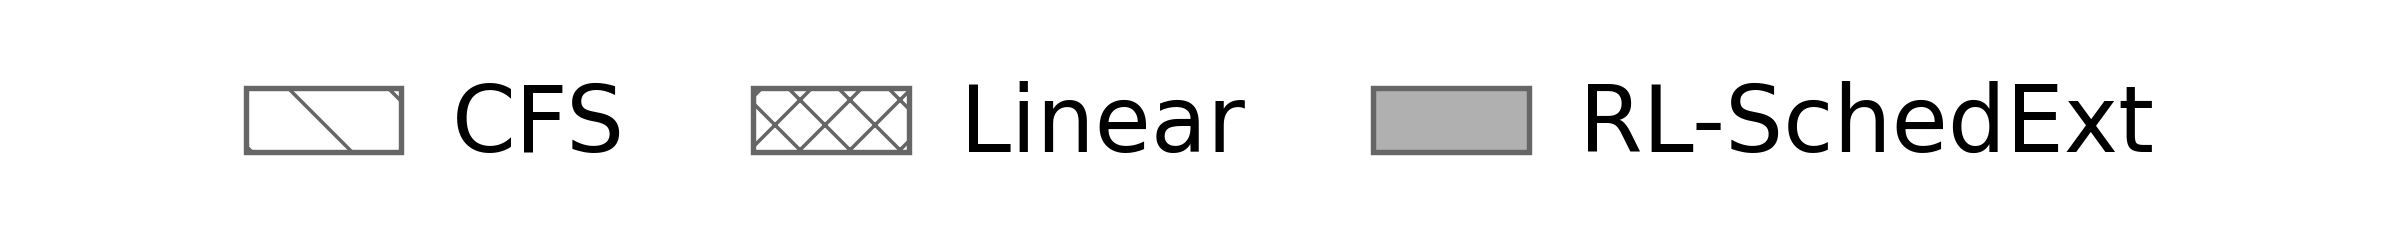
\includegraphics[width=0.50\linewidth]{Figures/fig5_2_legend.png}\par\smallskip
    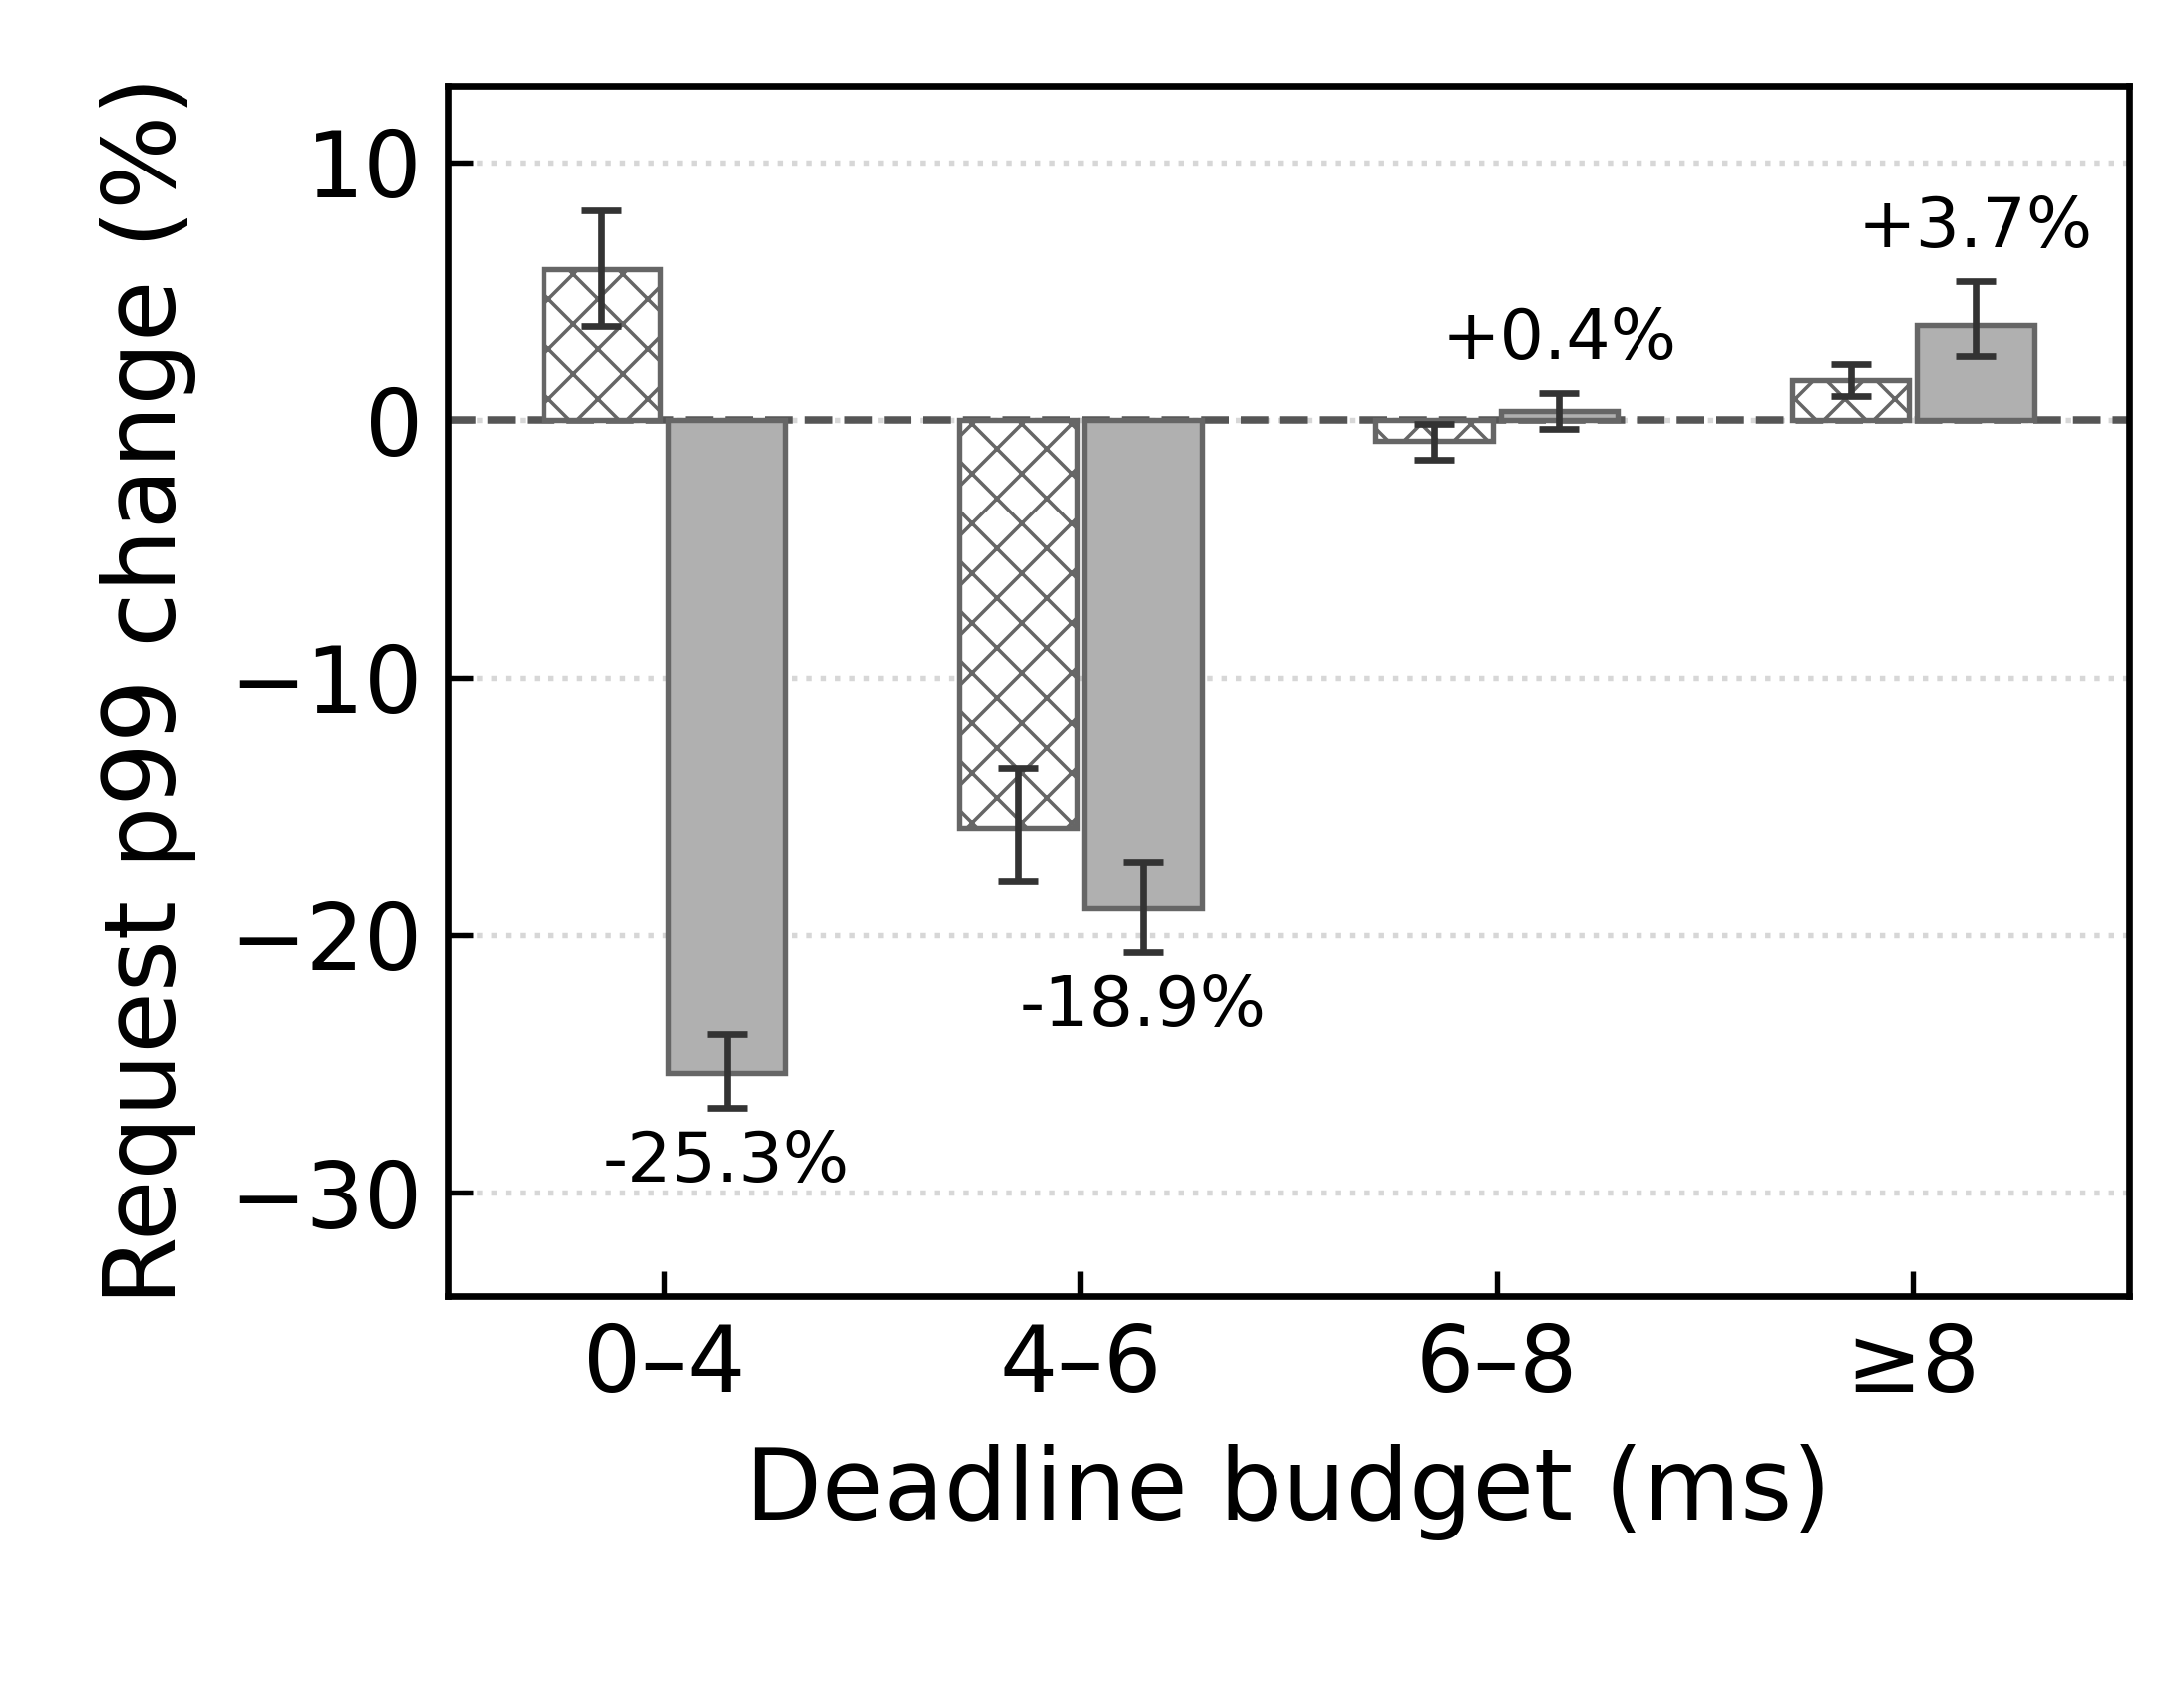
\includegraphics[width=0.65\linewidth]{Figures/fig5_2_mixed_p99_change.png}
    \caption{Mixed CPU Bursts에서 초기 Deadline Budget에 따른 Request Completion Latency p99의 변화율. 전체 100회의 측정 결과를 사용하였다. 점선은 CFS 기준값(0\%)을 나타내며, 오차 막대는 Bootstrap 95\% 신뢰구간을 나타낸다. 음의 변화율은 Latency 감소를 의미한다.}
    \label{fig:bimodal-p99-budget}
\end{figure}

이러한 결과는 Neural Student에서 Deadline Budget이 짧은 Request의
Completion Latency는 감소하는 반면, Deadline Budget이 상대적으로 긴 Request의
Completion Latency는 일부 증가하는 경향을 보여준다.
즉, Neural Student는 전체 Request Completion Latency를 균일하게 감소시키기보다
Scheduling Urgency를 고려하여 Task Ordering을 조정함으로써
Deadline Compliance를 향상시킨다.

\subsection{Analysis of Learned Vruntime Adjustment}
\label{sec:eval-analysis-of-learned-vruntime-adjustment}
앞선 실험에서는 Neural Student가 Linear Student보다 높은
Deadline Compliance를 달성하였다.
이러한 성능 차이를 분석하고 Task Ordering에 비선형 모델이 필요한
이유를 확인하기 위해, 두 Student가 Task의 Scheduling Urgency를
얼마나 효과적으로 구분하는지 평가하였다.

앞선 Microbenchmark와 동일한 Workload를 포함하여 각 Student에 대해
100회의 반복 실험을 수행하였다.
각 Scheduling Decision에서 Student는 관측 가능한 Task의 State를
기반으로 Learned Vruntime Adjustment를 결정한다.
그러나 실제 Scheduling 시점에는 Application Request의 Remaining Deadline을
알 수 없으므로, 각 Decision에서 생성된 Adjustment를 Kernel Trace로
수집하고 실험 종료 후 해당 Task가 처리하던 Request의 실제
Remaining Deadline과 Mapping하였다.

Figure~\ref{fig:deadline-relative-correction}은 실제 Remaining Deadline과
Relative Learned Vruntime Adjustment 사이의 관계를 보여준다.
동일한 Scheduling Decision에서 경쟁하는 Task 간의 상대적인
조정값을 비교하기 위해 각 Task의 Learned Vruntime Adjustment에서
Runnable Task Set의 평균 Learned Vruntime Adjustment를 차감하였다.
Scheduling Decision $k$의 Runnable Task Set을 $\mathcal{R}_k$라 하면,
분석에 사용하는 Relative Learned Vruntime Adjustment는 다음과 같다.

\begin{equation}
    \widetilde{\Delta V}_i =
    \Delta V_i -
    \frac{1}{|\mathcal{R}_k|}
    \sum_{j\in\mathcal{R}_k}\Delta V_j.
    \label{eq:relative_adjustment}
\end{equation}

이 값은 분석을 위해 계산한 값이며 실제 각 Student의 출력이나
Task Selection 방식을 변경하지 않는다.

\begin{figure}[H]
  \centering
  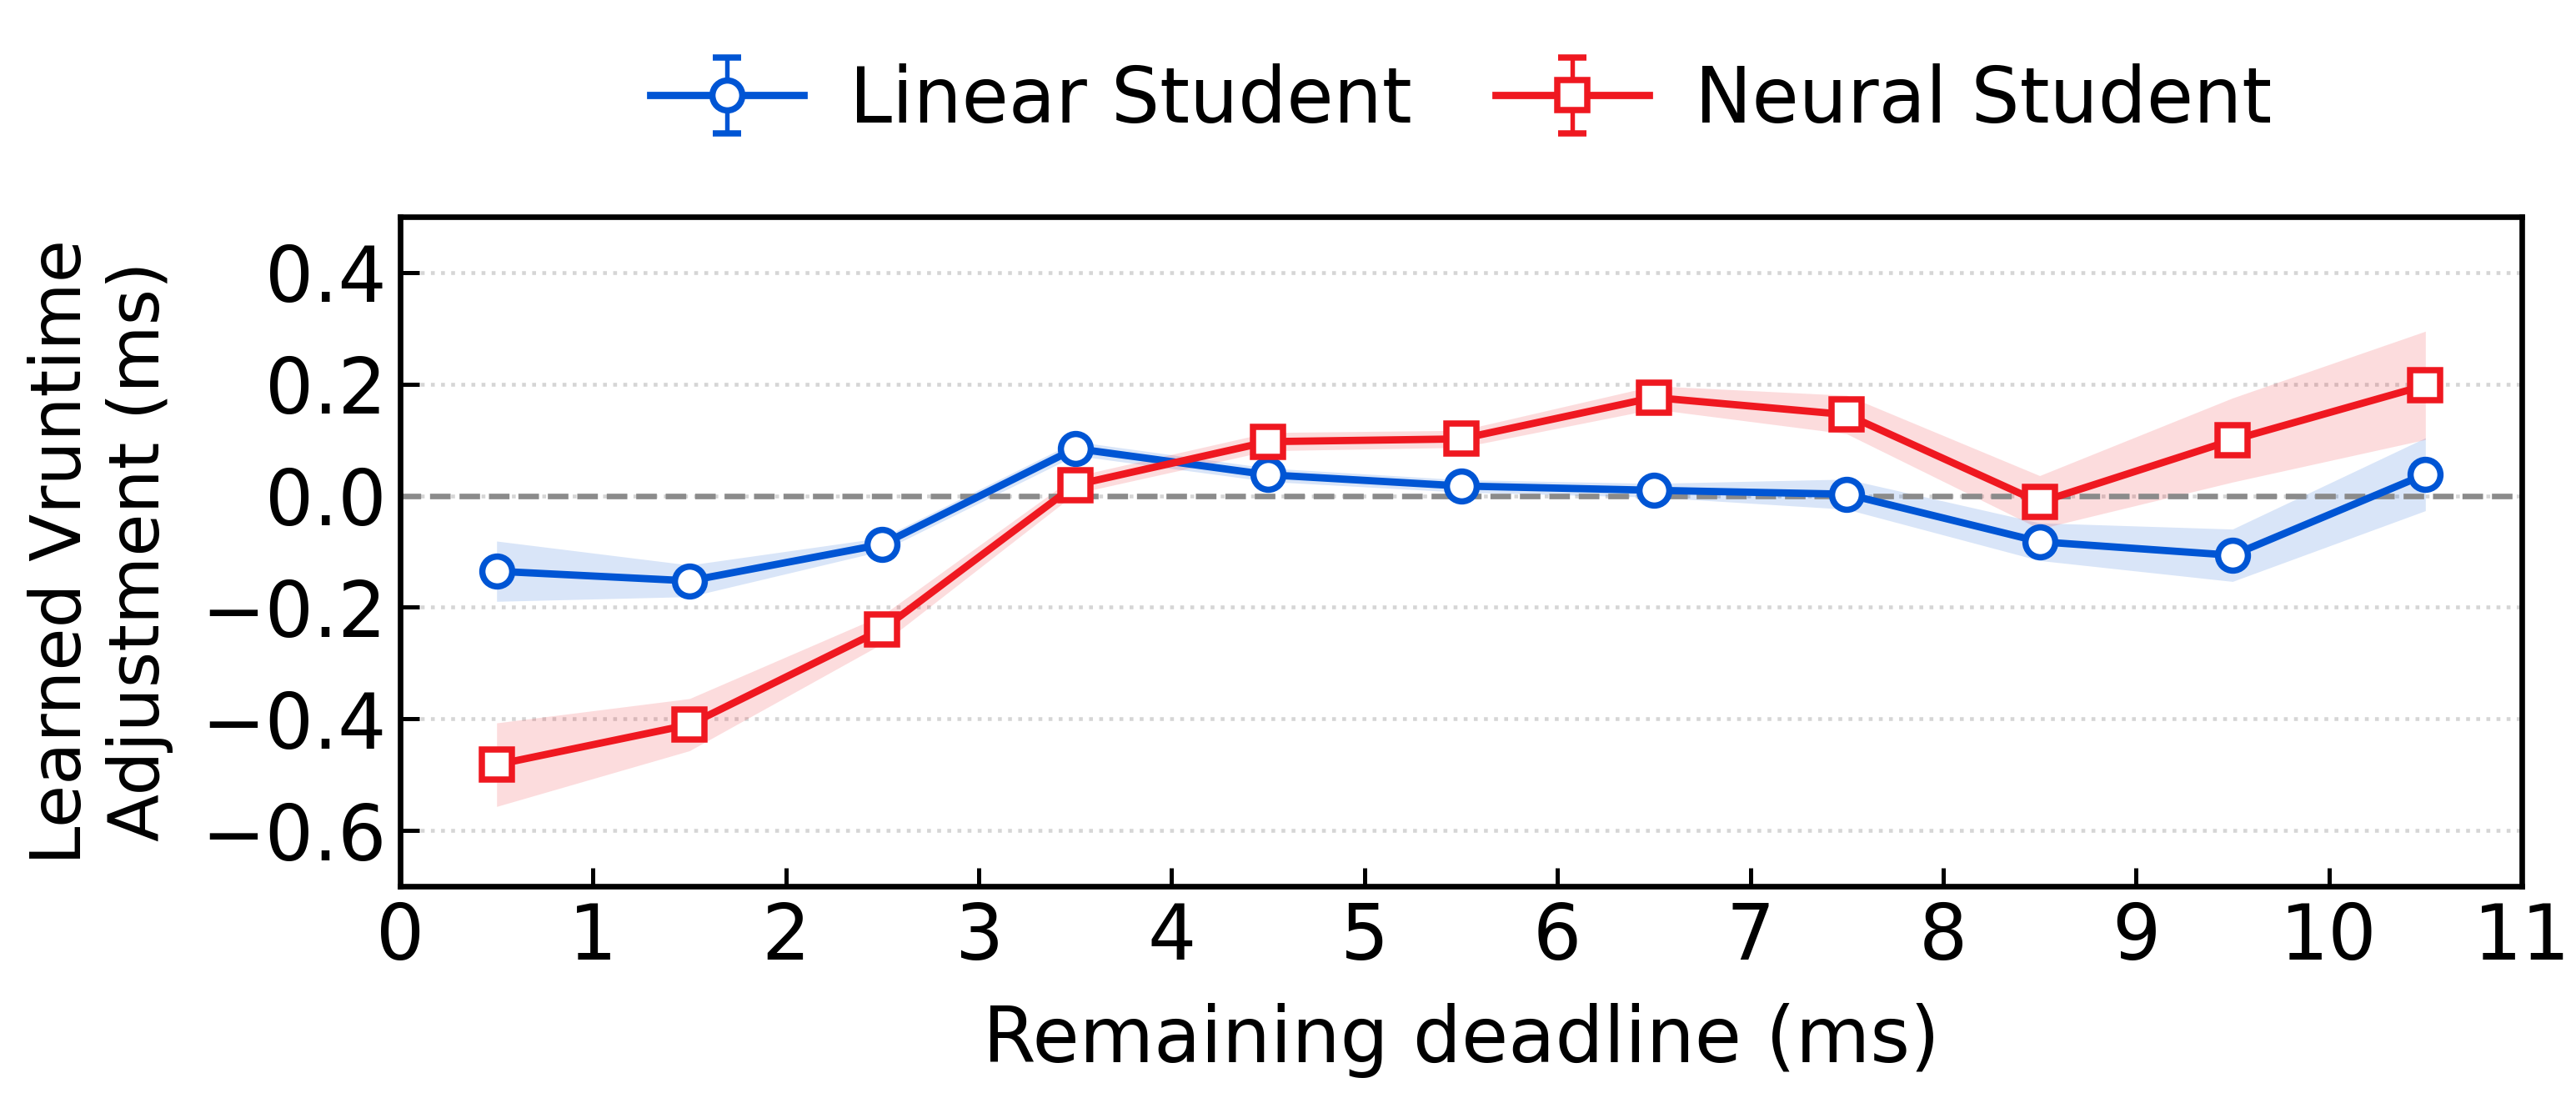
\includegraphics[width=0.82\linewidth]{Figures/fig5_3_deadline_adjustment.png}
  \caption{Remaining Deadline에 따른 Relative Learned Vruntime Adjustment.
  실선은 반복 실험 전체의 평균, 음영은 평균 $\pm$ 1 Standard Deviation,
  오차 막대는 95\% 신뢰구간을 나타낸다.}
  \label{fig:deadline-relative-correction}
\end{figure}

Neural Student의 Relative Learned Vruntime Adjustment는 처리 중인 Request의
Remaining Deadline이 0--1\,ms인 Task에서 평균 $-0.482$\,ms였으며,
6--7\,ms인 Task에서는 평균 $+0.176$\,ms였다.
두 구간의 Relative Learned Vruntime Adjustment 차이는 0.658\,ms로,
Linear Student의 0.145\,ms보다 약 4.5배 크게 나타났다.
이는 Neural Student가 Remaining Deadline이 짧은 Request를 처리하는 Task와
상대적으로 Remaining Deadline이 긴 Request를 처리하는 Task 사이에
더 큰 Relative Learned Vruntime Adjustment 차이를 보였음을 나타낸다.
이러한 결과는 실제 Deadline 정보가 제공되지 않는 환경에서
Neural Student가 관측 가능한 State로부터 Task의 Scheduling
Urgency를 Linear Student보다 효과적으로 추론함을 보여준다.
따라서 RL Teacher가 학습한 Context-dependent Task Ordering
특성을 유지하기 위해서는 단순한 선형 모델보다
비선형 모델을 사용하는 것이 효과적이다.

\section{Macrobenchmark}
\label{sec:eval-macrobenchmark}
\subsection{Workload and Methodology}
\label{sec:eval-workload-and-methodology}
실제 Android Application에서의 End-to-End 성능을 평가하기 위해 오픈소스 게임 \textit{Mindustry}를 단독으로 실행하였다~\cite{mindustry}. Mindustry는 게임 로직 처리와 렌더링이 동시에 수행되는 Android 게임으로, 게임 진행 상태와 사용자 조작에 따라 CPU 부하가 달라질 수 있다.

따라서 본 연구에서는 Scheduler 간 비교에서 Workload의 변동성을 최소화하기 위해 사전에 구성된 게임 저장 파일을 활용하였다. 60초 동안 Defense를 하는 시나리오를 수행하였으며, 게임의 시뮬레이션과 화면 갱신이 지속적으로 수행된다.

실험 결과는 60초 Defense 구간에서 수집한 SurfaceFlinger TimeStats를 이용하여 Average FPS와 Frame Interval Percentiles (p50, p95, p99)를 비교하였다. Average FPS는 단위 시간당 화면에 표시되는 프레임 수로, 게임의 전반적인 시각적 부드러움을 나타낸다. Frame Interval은 연속된 프레임의 실제 출력 시각 사이의 간격이며, 큰 Frame Interval은 간헐적인 화면 끊김과 Frame Pacing 불안정성을 나타낸다~\cite{timestats,framepacing}.
Mindustry와 같이 게임 로직과 렌더링이 지속적으로 수행되는 환경에서는 Average FPS가 유사하더라도 일부 프레임의 출력이 크게 지연되면 시각적 부드러움이 저하될 수 있다. 따라서 Average FPS뿐 아니라 Frame Interval의 Tail Latency를 함께 비교하여 일반적인 출력 성능과 긴 프레임 지연을 구분해 평가하였다.

실험은 CFS와 RL-SchedExt에 대해 각각 10회씩, 총 20회 반복하여 수행하였다. 매 실행마다 Application을 재시작함으로써 이전 실행에서 유지될 수 있는 게임 내부 상태의 영향을 최소화하고자 하였다. 최종 Average FPS와 Frame Interval은 각 Scheduler에서 측정한 10회 결과의 산술평균으로 산출하였다.


\subsection{Gaming Performance}
\label{sec:eval-gaming-performance}
Figure~\ref{fig:mindustry-macro}는 Mindustry 실행 환경에서 CFS와 RL-SchedExt의 Average FPS 및 Frame Interval을 비교한 결과이다. RL-SchedExt는 Average FPS 29.62를 기록하여 CFS의 26.47 대비 11.9\% 높은 성능을 보였다. 이는 동일한 게임 시나리오에서 단위 시간당 더 많은 프레임을 출력함으로써 게임의 전반적인 화면 갱신 성능을 향상시켰음을 의미한다.

\begin{figure}[H]
  \centering
  
\includegraphics[width=0.40\linewidth]{Figures/fig5_4_legend.png}\par\smallskip
  \captionsetup[subfigure]{skip=2pt}
  \begin{subfigure}[b]{0.39\linewidth}
    \centering
    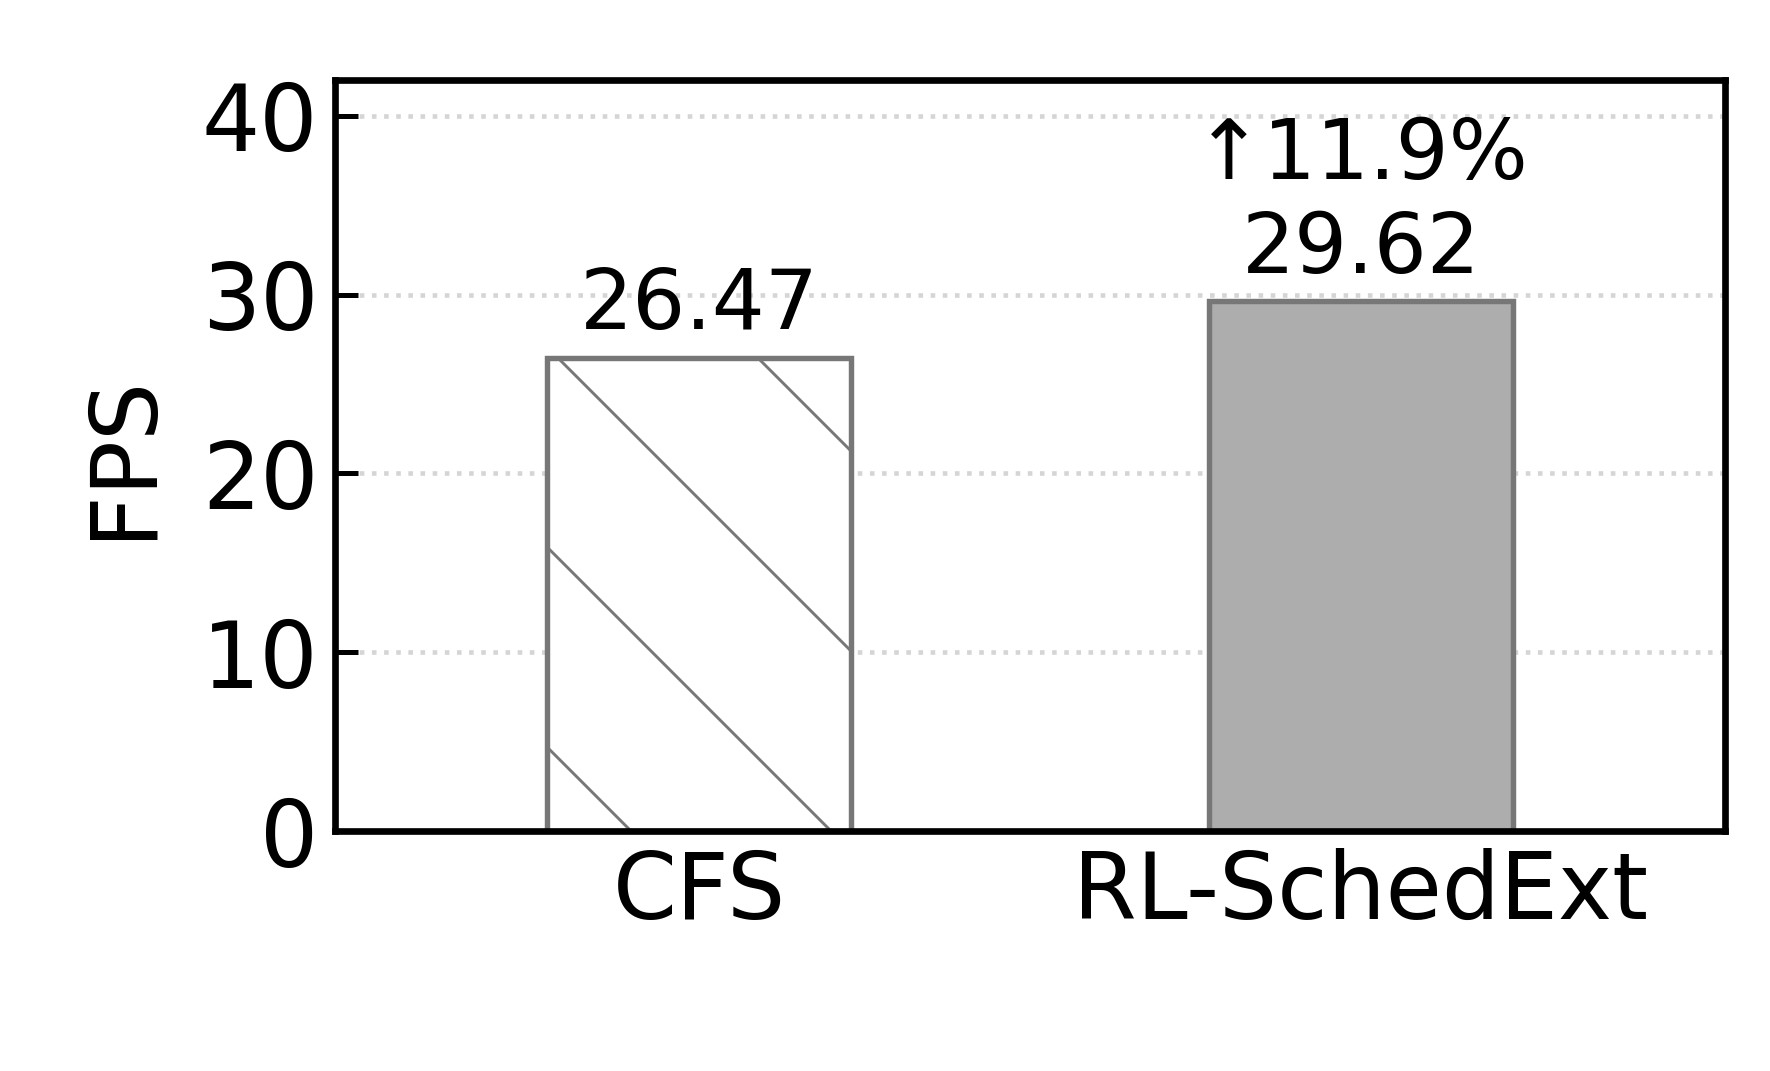
\includegraphics[width=\linewidth]{Figures/fig5_4_a_average_fps.png}
    \subcaption{Average FPS ($\uparrow$)}
    \label{fig:mindustry-fps}
  \end{subfigure}
  \hspace{2pt}%
  \begin{subfigure}[b]{0.575\linewidth}
    \centering
    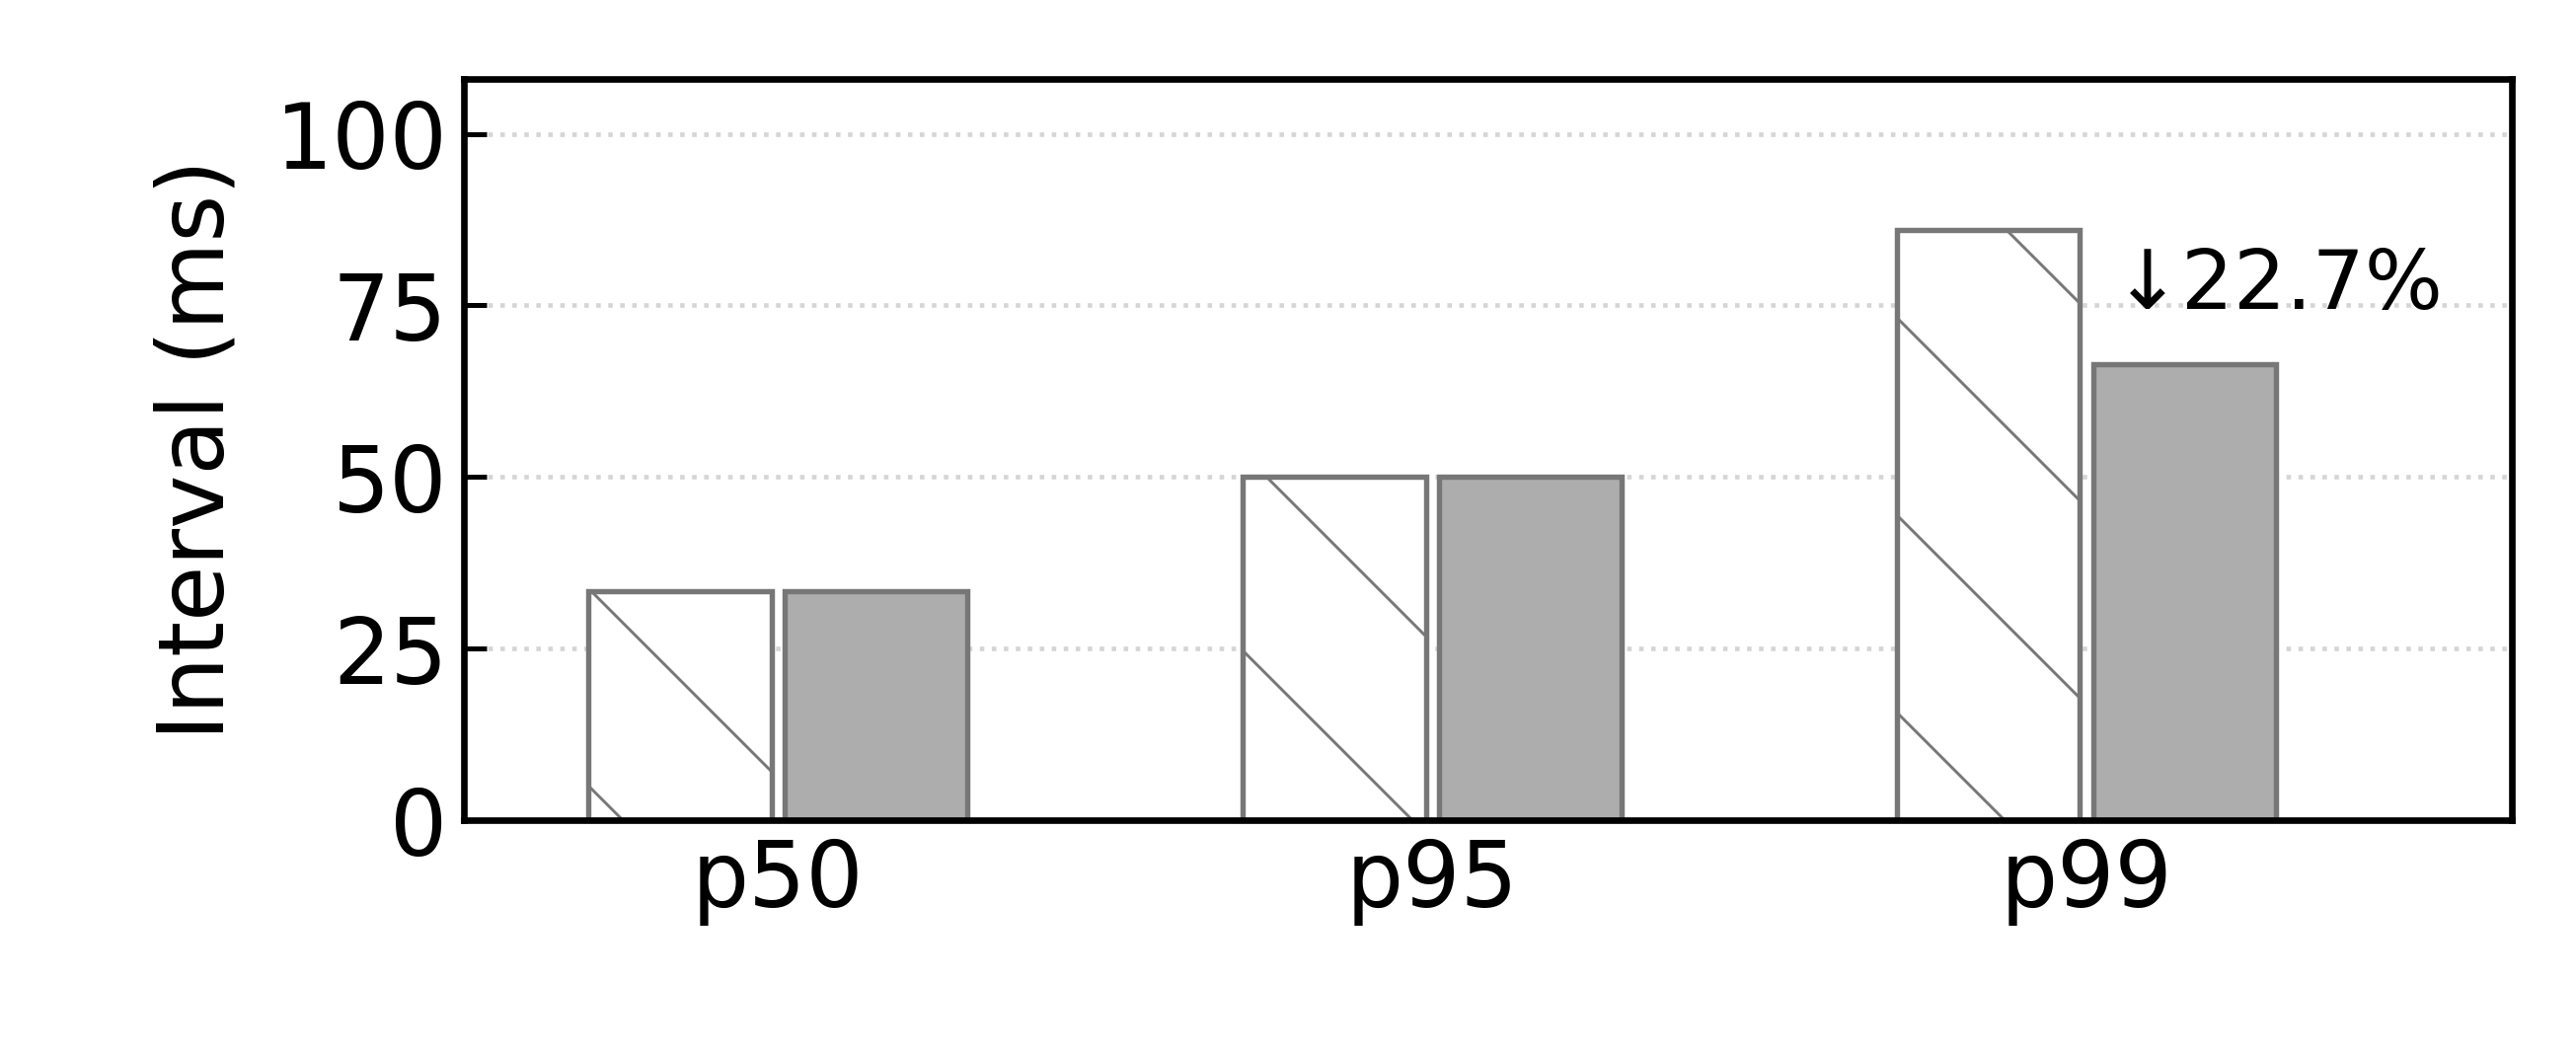
\includegraphics[width=\linewidth]{Figures/fig5_4_b_frame_interval.png}
    \subcaption{Frame Interval ($\downarrow$)}
    \label{fig:mindustry-interval}
  \end{subfigure}
  \caption{Mindustry 단독 실행에서 CFS와 RL-SchedExt의 게임 성능 비교. Frame Interval p50/p95/p99는 SurfaceFlinger의 게임 레이어 \texttt{present2present} 히스토그램을 기준으로 계산하였다.}
  \label{fig:mindustry-macro}
  \vspace{-0.7em}
\end{figure}

실험 결과, 두 Scheduler의 Frame Interval p50과 p95는 각각 33\,ms와 50\,ms로 동일하였으나, p99는 CFS의 86\,ms에서 RL-SchedExt의 66\,ms로 감소하여 23.3\% 감소하였다. 이는 일반적인 프레임 출력 간격은 유사하게 유지하면서도, 일부 프레임에서 발생하는 긴 출력 지연을 완화하였음을 보여준다.

종합하면, RL-SchedExt는 실제 Android Gaming Workload에서 Average FPS를 향상시키는 동시에 Frame Interval의 Tail Latency를 감소시켰다. 이러한 결과는 제안한 Scheduler가 게임의 전반적인 화면 갱신 성능뿐 아니라 간헐적인 화면 끊김(Stuttering)과 관련된 Frame Pacing 안정성도 개선할 수 있음을 보여준다.
